\newcommand{\badcell}[1]{\cellcolor{red!10}#1}
\newcommand{\goodcell}[1]{\cellcolor{green!10}#1}
\begin{figure}[!ht]
    \begin{minipage}[b]{.45\textwidth}
        \centering
        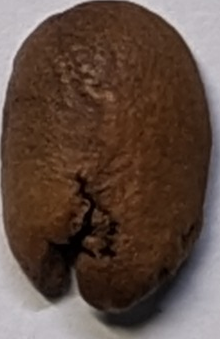
\includegraphics[height=\textwidth, angle=90, keepaspectratio]{classificationExamples/ethiopia-yirga-CM-frag-0-12}
        \subcaption{Actual class: fragmented/chipped bean}
        \label{fig:ex1}
    \end{minipage}
    \hfill
    \hspace{0.5em}
    \begin{minipage}[b]{.5\textwidth}
        \begin{tabular}{ll}
            \toprule
            \textbf{Classifier} & \textbf{Predicted class} \\
            \midrule
            \hyperref[tab:knnResults]{\hyperref[tab:knnResults]{KNN-2}}               & \goodcell{Fragmented/chipped}         \\
            \addlinespace[0.5em]
            \makecell[l]{MobileNet\\(no pre-training)} & \badcell{Quaker} \\
            \addlinespace[0.5em]
            \makecell[l]{MobileNet\\(pre-trained)}           & \badcell{Quaker}         \\
            \addlinespace[0.5em]
            ResNet 50           & \badcell{Quaker}         \\
            \bottomrule
        \end{tabular}
        \subcaption{Classifier predictions}
        \label{tab:ex1}
    \end{minipage}
    \caption{}
\end{figure}

While the human eye can easily spot the crack on the left side of the bean, the neural networks may have struggled to do so
due to a lack of illumination of the crack.
The lack of light may have made it difficult to tell the crack apart from a dark surface marking, which are associated with
the ''quaker`` class, confusing the neural networks.

The KNN classifier correctly identified this bean, which was most likely caused by the dataset containing several other beans
with shallow cracks, making this bean's colour histogram match that of the others.

This case reflects the need for stronger lighting and/or higher resolution when taking the images and identifies an area
of future improvement.
\pagebreak
\begin{figure}[!ht]
    \begin{minipage}[b]{.45\textwidth}
        \centering
        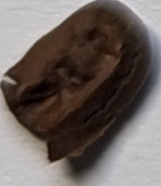
\includegraphics[height=\textwidth, angle=270, keepaspectratio]{classificationExamples/brazil-wushwush-nat-frag-0-5}
        \subcaption{Actual class: fragmented/chipped bean}
        \label{fig:ex2}
    \end{minipage}
    \hfill
    \hspace{0.5em}
    \begin{minipage}[b]{.5\textwidth}
        \begin{tabular}{ll}
            \toprule
            \textbf{Classifier} & \textbf{Predicted class}      \\
            \midrule
            \hyperref[tab:knnResults]{KNN-2}               & \badcell{Normal}              \\
            \addlinespace[0.5em]
            \makecell[l]{MobileNet\\(no pre-training)} & \goodcell{Fragmented/chipped} \\
            \addlinespace[0.5em]
            \makecell[l]{MobileNet\\(pre-trained)}           & \goodcell{Fragmented/chipped} \\
            \addlinespace[0.5em]
            ResNet 50           & \goodcell{Fragmented/chipped} \\
            \bottomrule
        \end{tabular}
        \subcaption{Classifier predictions}
        \label{tab:ex2}
    \end{minipage}
    \caption{}
\end{figure}

This bean highlights the weakness of the histogram method used for the KNN classifier: while this bean is clearly misshapen
and fragmented, its relatively uniform colour made the KNN classifier assign it the ''normal`` class.

On the other hand, the rough edges and uneven surface of this bean were easily spotted by all neural networks, leading to
a correct prediction.

\begin{figure}[!ht]
    \begin{minipage}[b]{.45\textwidth}
        \centering
        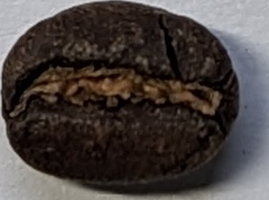
\includegraphics[width=\textwidth]{classificationExamples/ethiopia-ethHeirloom-washed-normal-15-12}
        \subcaption{Actual class: normal}
        \label{fig:ex3}
    \end{minipage}
    \hfill
    \hspace{0.5em}
    \begin{minipage}[b]{.5\textwidth}
        \begin{tabular}{ll}
            \toprule
            \textbf{Classifier} & \textbf{Predicted class} \\
            \midrule
            \hyperref[tab:knnResults]{KNN-2}               & \badcell{Quaker}         \\
            \addlinespace[0.5em]
            \makecell[l]{MobileNet\\(no pre-training)} & \goodcell{Normal} \\
            \addlinespace[0.5em]
            \makecell[l]{MobileNet\\(pre-trained)}           & \goodcell{Normal}        \\
            \addlinespace[0.5em]
            ResNet 50           & \goodcell{Normal}        \\
            \bottomrule
        \end{tabular}
        \subcaption{Classifier predictions}
        \label{tab:ex3}
    \end{minipage}
    \caption{}
\end{figure}

The misclassification of the KNN model here can be explained by the strip of ''chaff`` (dried husk of the coffee cherry)
that did not get removed during the roasting process and has little to no effect on the final product.

While the neural networks correctly identified the surface texture and dark colour as those of a normally roasted bean,
the lighter strip may have skewed the colour distribution of the image, bringing the bean closer to ''quaker`` beans, which
tend to have a lighter colour due to their lack of sugar not enabling them to caramelize.

\begin{figure}[!ht]
    \begin{minipage}[b]{.45\textwidth}
        \centering
        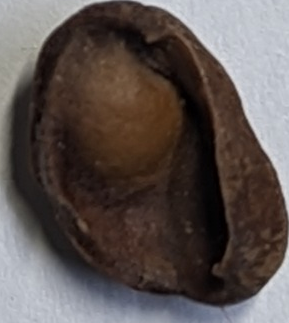
\includegraphics[height=\textwidth, angle=90]{classificationExamples/kenya-sl28-washed-frag-1-8}
        \subcaption{Actual class: fragmented/chipped bean}
        \label{fig:ex4}
    \end{minipage}
    \hfill
    \hspace{0.5em}
    \begin{minipage}[b]{.5\textwidth}
        \begin{tabular}{ll}
            \toprule
            \textbf{Classifier} & \textbf{Predicted class}      \\
            \midrule
            \hyperref[tab:knnResults]{KNN-2}               & \badcell{Normal}              \\
            \addlinespace[0.5em]
            \makecell[l]{MobileNet\\(no pre-training)} & \goodcell{Fragmented/chipped} \\
            \addlinespace[0.5em]
            \makecell[l]{MobileNet\\(pre-trained)}           & \goodcell{Fragmented/chipped} \\
            \addlinespace[0.5em]
            ResNet 50           & \goodcell{Fragmented/chipped} \\
            \bottomrule
        \end{tabular}
        \subcaption{Classifier predictions}
        \label{tab:ex4}
    \end{minipage}
    \caption{}
\end{figure}

The image here displays similar traits to that in figure~\ref{fig:ex3}, with a relatively even colour distribution confusing
the KNN classifier.

On the other hand, the neural networks were able to detect the likely features of a bean fragment, such as the sharp edges
on the top and left of the bean.
\begin{figure}[!ht]
    \begin{minipage}[b]{.45\textwidth}
        \centering
        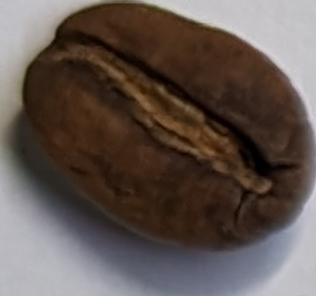
\includegraphics[width=\textwidth]{classificationExamples/ethiopia-yirga-CM-quaker-1-19}
        \subcaption{Actual class: quaker}
        \label{fig:ex5}
    \end{minipage}
    \hfill
    \hspace{0.5em}
    \begin{minipage}[b]{.5\textwidth}
        \begin{tabular}{ll}
            \toprule
            \textbf{Classifier} & \textbf{Predicted class} \\
            \midrule
            \hyperref[tab:knnResults]{KNN-2}               & \badcell{Normal}         \\
            \addlinespace[0.5em]
            \makecell[l]{MobileNet\\(no pre-training)} & \goodcell{Quaker} \\
            \addlinespace[0.5em]
            \makecell[l]{MobileNet\\(pre-trained)}           & \goodcell{Quaker}         \\
            \addlinespace[0.5em]
            ResNet 50           & \goodcell{Quaker}         \\
            \bottomrule
        \end{tabular}
        \subcaption{Classifier predictions}
        \label{tab:ex5}
    \end{minipage}
    \caption{}
\end{figure}

This bean, with its lighter colour and occasional dark patches, showcases the typical signs of a ''quaker`` bean.
Despite this, the image contains a relatively large shadow, which could have skewed the colour distribution towards darker
shades, affecting the judgement of the KNN classifier.
On the other hand, all neural network classifiers were able to extract more information from the image, possibly making use
of its textures and shapes, as well as the colours, making the correct prediction.
\pagebreak
\begin{figure}[!ht]
    \begin{minipage}[b]{.45\textwidth}
        \centering
        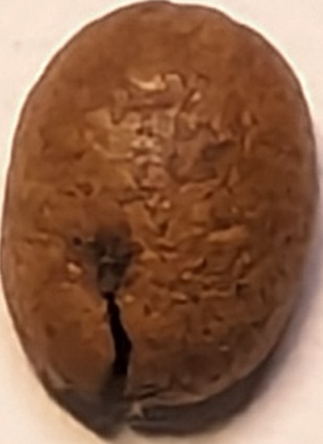
\includegraphics[height=\textwidth, angle=270]{classificationExamples/ethiopia-yirga-CM-insect-2-1}
        \subcaption{Actual class: insect/mould damage}
        \label{fig:ex6}
    \end{minipage}
    \hfill
    \hspace{0.5em}
    \begin{minipage}[b]{.5\textwidth}
        \begin{tabular}{ll}
            \toprule
            \textbf{Classifier} & \textbf{Predicted class} \\
            \midrule
            \hyperref[tab:knnResults]{KNN-2}               & \goodcell{Insect/mould}  \\
            \addlinespace[0.5em]
            \makecell[l]{MobileNet\\(no pre-training)} & \badcell{Quaker} \\
            \addlinespace[0.5em]
            \makecell[l]{MobileNet\\(pre-trained)}           & \badcell{Quaker}  \\
            \addlinespace[0.5em]
            ResNet 50           & \goodcell{Insect/mould}  \\
            \bottomrule
        \end{tabular}
        \subcaption{Classifier predictions}
        \label{tab:ex6}
    \end{minipage}
    \caption{}
\end{figure}

The insect damage in this bean is localised to a dark spot near its center.
A crack caused by the damage can also be seen towards the left, which, as seen in other examples here, communicates little
texture information due to a lack of illumination.
Because of this, it can be surmised that this crack can instead be seen as a surface mark on a ''quaker`` bean, confusing the
MobileNet classifiers.
The ResNet classifier's larger number of parameters is the likely reason for its success, allowing it to develop more thorough
internal descriptions of input images.

\begin{figure}[!ht]
    \begin{minipage}[b]{.45\textwidth}
        \centering
        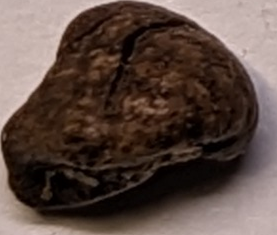
\includegraphics[width=\textwidth]{classificationExamples/ethiopia-guji-washed-frag-0-1}
        \subcaption{Actual class: fragmented/chipped bean}
        \label{fig:ex7}
    \end{minipage}
    \hfill
    \hspace{0.5em}
    \begin{minipage}[b]{.5\textwidth}
        \begin{tabular}{ll}
            \toprule
            \textbf{Classifier} & \textbf{Predicted class}      \\
            \midrule
            \hyperref[tab:knnResults]{KNN-2}               & \goodcell{Fragmented/chipped} \\
            \addlinespace[0.5em]
            \makecell[l]{MobileNet\\(no pre-training)} & \badcell{Quaker} \\
            \addlinespace[0.5em]
            \makecell[l]{MobileNet\\(pre-trained)}           & \badcell{Burnt}        \\
            \addlinespace[0.5em]
            ResNet 50           & \badcell{Insect/mould}        \\
            \bottomrule
        \end{tabular}
        \subcaption{Classifier predictions}
        \label{tab:ex7}
    \end{minipage}
    \caption{}
\end{figure}
The bean in this example is severely misshapen and fragmented, with a large crack seen on its top surface.
Furthermore, the bean appears to have a normal sugar content, which can be deducted from its dark and relatively even
surface.
The image of the bean lacks any sharp edges and contains shadows, a combination of factors
that could have influenced the judgements of both MobileNet based classifiers.
The decision of the ResNet classifier can possibly be explained by a darker region on the bottom left of the bean, which
resembles the holes left behind by insects.

Overall, the colour distribution shift caused by the cracks and shadows can explain the correct prediction of the KNN
classifier, though this is unlikely to generalise well to other such beans.
\begin{figure}[!ht]
    \begin{minipage}[b]{.45\textwidth}
        \centering
        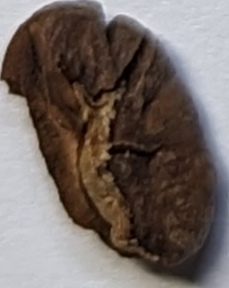
\includegraphics[height=\textwidth, angle=270]{classificationExamples/kenya-sl28-washed-frag-0-6}
        \subcaption{Actual class: fragmented/chipped bean}
        \label{fig:ex8}
    \end{minipage}
    \hfill
    \hspace{0.5em}
    \begin{minipage}[b]{.5\textwidth}
        \begin{tabular}{ll}
            \toprule
            \textbf{Classifier} & \textbf{Predicted class} \\
            \midrule
            \hyperref[tab:knnResults]{KNN-2}               & \badcell{Normal}         \\
            \addlinespace[0.5em]
            \makecell[l]{MobileNet\\(no pre-training)} & \badcell{Quaker} \\
            \addlinespace[0.5em]
            \makecell[l]{MobileNet\\(pre-trained)}           & \goodcell{Fragmented/chipped}         \\
            \addlinespace[0.5em]
            ResNet 50           & \badcell{Quaker}         \\
            \bottomrule
        \end{tabular}
        \subcaption{Classifier predictions}
        \label{tab:ex8}
    \end{minipage}
    \caption{}
\end{figure}

While the misprediction of the KNN classifier can be explained by the overall colour distribution of this bean, it is also
clear that the CNN classifiers also had difficulty in identifying this bean's defect.
The likely reason behind the mispredictions stems from the bean exhibiting several defects at once, with both a shrivelled
surface commonly associated with ''quaker`` beans, and sharp edges and cracks associated with bean fragments.
This edge case shows a need for further example of beans exhibiting several defects at once, which can be done in future versions
of the dataset.

\section{Raw misclassification results}
\label{sec:raw-misclassification-results}
The raw results are available in the project submission archived folder, under the following path: \\
\verb|implementation/misclassified_results.json|